\chapter{Evaluation}
\label{chp:evaluation}

We address RQ1 by proposing entities (discussed in \chp{chp:approach}) to be
instantiated
in multimedia languages. After doing so, we have also proposed syntax
instantiations for NCL and HTML (discussed in \chp{chp:instantiation}).

Nowadays, the development of NCL and HTML applications can be done using
different approaches and representations. For instance, today NCL provide
alternative representations to its XML syntax, such as JSON objects
~\cite{silva_jns:_2013} and Lua tables~\cite{moraes_lua2ncl:_2016}. Moreover,
it is possible to develop in HTML using some alternative representations, such
as in XML (\textit{i.e.}~XHTML) and YAML, or even to use only JavaScript to
create the entire HTML DOM.

Given the above context, to evaluate our answer, we confront an additional
question about \textit{“how to evaluate the usage of the proposed entities
despite the different ways of instantiating them in a multimedia language?”}.
In other words, if we only evaluate the usage of our proposed syntax, the
evaluation results will be tied to the syntax development characteristics. For
the NCL syntax, for instance, Soares Neto \textit{et
al.}~\cite{de_salles_soares_neto_linguagens_2008}
performed a usability analysis and highlighted NCL verbosity and error-prone
characteristics. To answer such question, we performed an evaluation organized
in two parts. The first part focuses on the conceptual entities, whereas the
second part focuses on our proposed syntaxes for HTML and NCL.

Planning the analysis for the conceptual entities was a challenge, because they
were created to be independent from representation syntax. To do so, we used a
block-based programing paradigm to enable users to develop applications using
only the concept entities, at a level of abstraction higher than that of either
NCL or HTML. This paradigm is commonly used for teaching programming or in code
generation tools. In particular, this type of development has been popularized
by tools such as MIT Scratch\footnotemark and MIT App Inventor\footnotemark.
Although our block representation also contains its own syntax, a block syntax
helps users to abstract away from specificities and lower-level textual syntax
of the languages~\cite{shapiro_beyond_2016}, helping developers to focus on the
concepts we wish to evaluate.

\footnotetext[1]{\url{https://scratch.mit.edu/}}
\footnotetext[2]{\url{appinventor.mit.edu/}}

The analyses were performed with NCL and HTML developers through a web-based
evaluation form. This form not carry an execution runtime for the application,
i.e., the developers not visualize the multimedia application results; it focus
only in presents model entities in the block-based and in extended language
representations to capture their understanding and acceptance by the
developers. In the next sections, we briefly present our block-based
representation (\subsect{sec:evaluation:blocks}), detail our evaluation form
(\subsect{sec:evaluation:form}), and discuss the results
(\subsect{sec:evaluation:discussion}).

\section{Block-based representation}
\label{sec:evaluation:blocks}

Our block representation was developed using the web-based version of the
Blockly\footnotemark framework. In this framework, the blocks are defined as
JavaScript
objects and then instantiated as SVG elements in HTML DOM. Then, those blocks as
SVG elements are showed in a workspace <div>, where the user can drag and drop
elements, fill in some fields, and join elements together. We have created four
group blocks, each one related with one entity.

\footnotetext{\url{https://developers.google.com/blockly/}}

In our block representation, a \textit{Media} entity is defined by joining a
media block, with the id field filled in, and a media content block, which can
be an image, audio, video or speech synthesis block. Similar, a Recognizer
entity is defined by joining a recognizer block, with the id field filled in,
and a recognized content block, which can be a speech or hand gesture block.
\fig{fig:blocksgroups} illustrates the block groups related with the
\textit{Media},
\textit{Recognizer} and
\textit{UserClass} entities.

\begin{figure}[!ht]
\begin{center}
	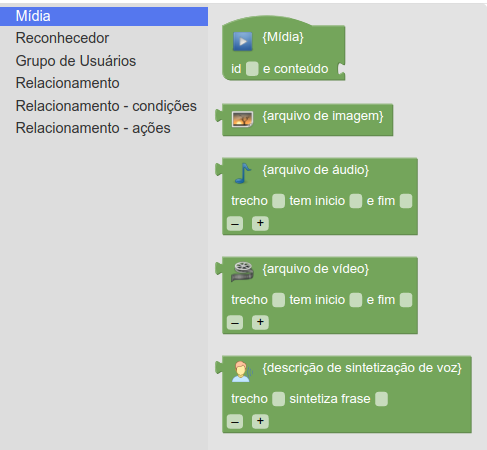
\includegraphics[width=4.4cm, keepaspectratio]{img/img13a.png}
	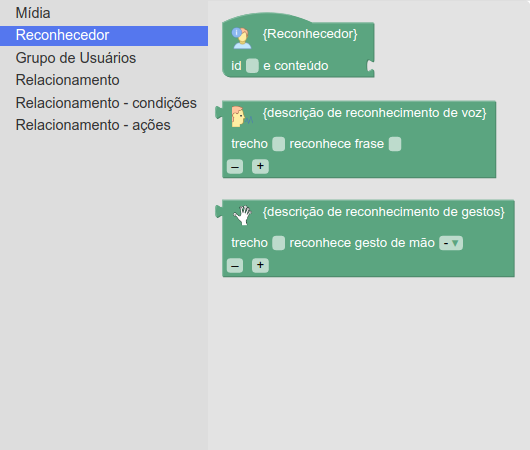
\includegraphics[width=4.4cm, keepaspectratio]{img/img13b.png}
	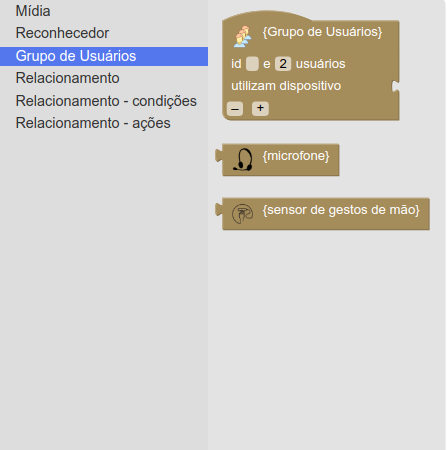
\includegraphics[width=4.4cm, keepaspectratio]{img/img13c.png}
	\caption{Blocks groups related to \textit{Media}, \textit{Recognizer} and
	\textit{UserClass}.}
	\label{fig:blocksgroups}
	\captionvspace
\end{center}
\end{figure}

A \textit{Relationship} is defined by joining one \textit{Relationship} block
with conditions and action blocks. Condition blocks can be simple or
compound. Simple condition blocks can define the trigger for: begin or end of
media/recognizer anchor or block id; selection of media block; recognition of
recognizer anchor or block id. A compound condition block allows combining other
condition blocks and use a combination operator (“OR”, “AND”, “SEQ”). Finally,
the action blocks can be start or stop a media/recognizer anchor or block id.
\fig{fig:blocks1} illustrates the blocks related with the \textit{Relationship}
entity. To prevent users from having the fill in all id values, the fields in
these \textit{Relationship} blocks are dropdowns, which list the existing
media/recognizer anchor or block ids.

\begin{figure}[!ht]
\begin{center}
	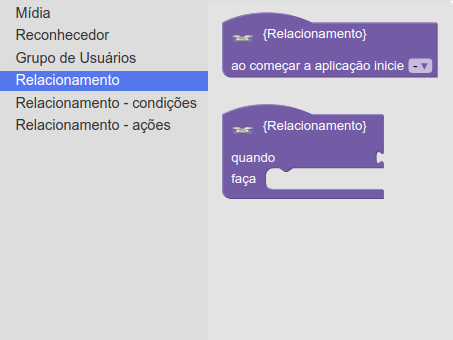
\includegraphics[width=4.4cm, keepaspectratio]{img/img14a.png}
	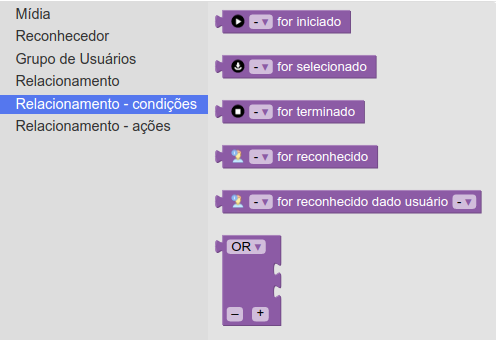
\includegraphics[width=4.4cm, keepaspectratio]{img/img14b.png}
	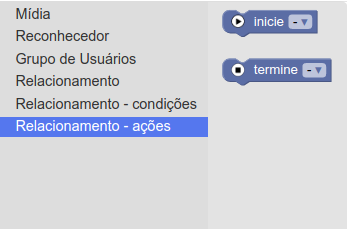
\includegraphics[width=4.4cm, keepaspectratio]{img/img14c.png}
	\caption{Blocks groups related to \textit{Relationship} related.}
	\label{fig:blocks1}
	\captionvspace
\end{center}
\end{figure}

To illustrate the usage of our block representation, \fig{fig:blocks2} presents
the “Multimodal Sightseeing of Today” application. It defines four
\textit{Media} and one
\textit{Recognizer} (left part of \fig{fig:blocks2}).

\begin{figure}[!ht]
  \begin{center}
    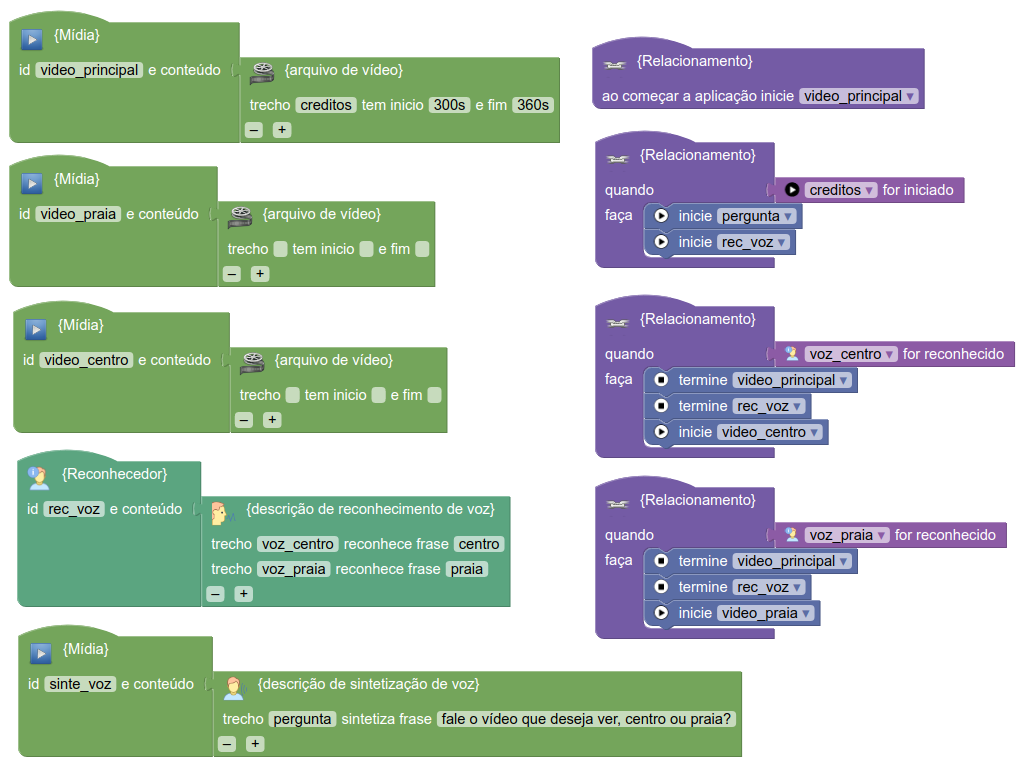
\includegraphics[width=14cm, keepaspectratio]{img/img15.png}
    \captionvspace
    \caption{Block-based representation of “Multimodal Sightseeing of Today”.}
    \captionvspace
    \label{fig:blocks2}
  \end{center}
\end{figure}

The first three \textit{Media} elements (“video\_principal”, “video\_praia” and
“video\_centro”) define the introductory video and the two videos available for
the user to choose from. The
“intro” video has an anchor (“creditos”) starting at 300 seconds in the video.
The last \textit{Media} (“sinte\_voz”) defines a speech synthesis media asking about the
navigation control. Finally, the \textit{Recognizer} (“asr\_places”) defines the
speech recognition for navigation control. This \textit{Recognizer} defines two
anchors, mapping onto the words “centro” and “praia”.

Regarding the application behavior, we define four \textit{Relationship}s (right
part of the \fig{fig:blocks2}): The first one defines that the application
begins by starting the “video\_principal” video. The second one defines that,
when the “creditos” anchor is reached, then the application asks for possible
places via voice commands. The other one defines that, when the user says the
name of a recognized place, then the corresponding video should be started.

\section{Evaluation form}
\label{sec:evaluation:form}

Our evaluation form aimed at capturing from NCL and HTML developers’ indications
of their acceptance of our proposal. More precisely, the form presents
questionnaires about both representations of our entities using the block-based
and language syntax representations. Our questionnaires were based in the
Technology Acceptance Model (TAM)~\cite{davis_perceived_1989}.

TAM is based on empirical studies and argues that users’ acceptance of a
technology is influenced mainly by the perceived usefulness (PU) and the
perceived ease of use (PEOU) of the technology. In our evaluation form, we
defined PU and PEOU questions guided by Gefen’s and Keil’s
~\cite{gefen_impact_1998} examples for both block-based and language
representations. However, TAM only captures the users’ perception and not their
actual understanding of a technology. To overcome this issue, we not only
presented the representations but we asked users to perform tasks using them.

The evaluation study comprised 37 participants. In our analyses, we organize
them into two groups based on their self-assessment of their knowledge of NCL
and HTML. As we expected to have more volunteers knowledgeable in HTML, if a
participant answered had the same degree of knowledge in both languages, we
allocated him/her to the NCL group. We ended up with 21 participants in the HTML
group and 16 in the NCL group. Because of the different sizes of the groups, all
charts presented in this section use percentages to inform the proportion of
participants inside each group gave a certain answer. The evaluation form is
organized in seven pages. The first five pages target all participants, because
they introduce concepts, ask profile questions and use the block-based
representation. The last two pages are adapted given the participant main
language. The participant answers questions about the extended NCL syntax if
he/she belongs to the NCL group. Conversely, he/she answers questions about the
extended HTML syntax if he/she belongs to the HTML group. The evaluation form
pages are listed in what follows. For a complete detail of the form and its
questions, we refer the reader to \appen{annex:screenshots}, which presents screenshots of
all pages.

\begin{itemize}
	\item Page 1 for all participants introduces the evaluation form and ask for
	the participants’ consent to participate in the study;
	\item Page 2 for all participants introduces multimedia languages with
	multimodal and multiuser features. In particular, it shows
	\fig{fig:overview-multimedia} and \fig{fig:overview-multimodal} to distinguish
	languages with and without such features;
	\item Page 3 for all participant presents profile questions;
	\item Page 4 for all participants presents the block-based representation and
	its tasks;
	\item Page 5 for all participants presents TAM questions about the entities of
	the conceptual model;
	\item Page 6 for NCL participants presents the extended NCL syntax and its
	tasks. We also organize this page like Page 4 (same entities and tasks) but
	using our extended NCL syntax.
	\item Page 7 for NCL participants presents TAM questions about the extended
	NCL syntax;
	\item Page 6 for HTML participants presents the extended HTML syntax and its
	tasks. We also organize this page like the Page 4 (same entities and tasks)
	but using our extended HTML syntax;
	\item Page 7 for HTML participants presents TAM questions about the extended
	HTML syntax.
\end{itemize}

In the next subsections, we detail and discuss the evaluation results. First, we
present the participants’ profiles (\subsect{sec:evaluation:profile-res}).
Then, we discuss their tasks and TAM answers related to the block-based
(\subsect{sec:evaluation:blocks-res}) and to the syntax-based representation
(\subsect{sec:evaluation:lang-res}).

\subsection{Participants’ profiles }
\label{sec:evaluation:profile-res}

The results of the profile questions enable us to characterize that most of the
participants are developers with postgraduate degrees and skilled in their group
language (NCL or HTML). More precisely, \fig{fig:profile1} shows that most
participants have a background in Computer Science, whereas as
\fig{fig:profile2} shows that they mainly consider themselves as skilled
(moderate to expert answers) in their group language. To understand their skill,
we also asked how many applications they developed in their language group and
most of them had developed more than eight applications (illustrated in
\fig{fig:profile3}).

Regarding their multimodal development skill, few participants had developed
multimodal applications at the time of the study (\fig{fig:profile4}). Among
those that had developed, we ask which kind application and most of them said
that had created some application for the Microsoft Kinect sensor.

\begin{figure}[!ht]
\begin{center}
	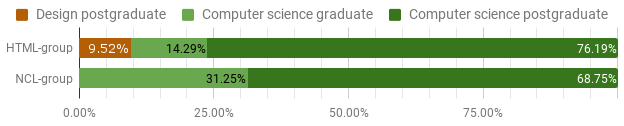
\includegraphics[width=10cm, keepaspectratio]{img/img16.png}
	\caption{Participants’ answers about their educational background.}
	\label{fig:profile1}
    \captionvspace
\end{center}
\end{figure}

\begin{figure}[!ht]
\begin{center}
	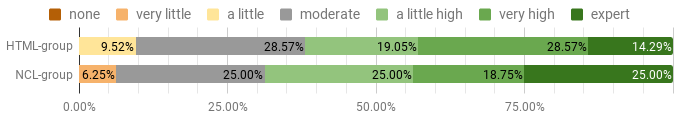
\includegraphics[width=10cm, keepaspectratio]{img/img17.png}
	\caption{Participants’ answers about their skill in their group language.}
	\label{fig:profile2}
    \captionvspace
\end{center}
\end{figure}

\begin{figure}[!ht]
\begin{center}
	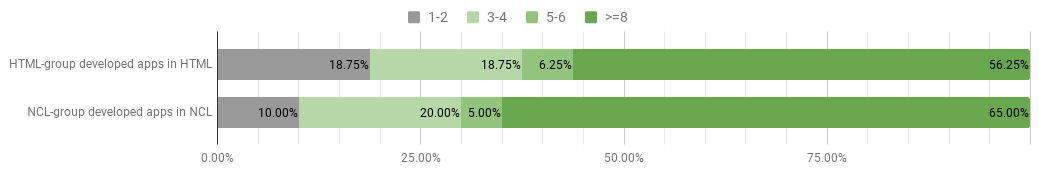
\includegraphics[width=14cm, keepaspectratio]{img/img18.png}
	\caption{Participants’ answers about the number of development applications
	in their main language.}
	\label{fig:profile3}
    \captionvspace
\end{center}
\end{figure}


\begin{figure}[!ht]
\begin{center}
	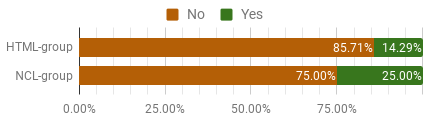
\includegraphics[width=8cm, keepaspectratio]{img/img19.png}
	\caption{Participants’ answers about whether they had developed multimodal
	applications.}
    \captionvspace
	\label{fig:profile4}
\end{center}
\end{figure}

\subsection{Results about block-based representations}
\label{sec:evaluation:blocks-res}

Page 4 of the evaluation form presents the block-based representation and is
organized in four sections; each one presents a few concepts, followed by a
task.

\begin{itemize}
	\item Concepts 1.1: Presents the \textit{Media} and \textit{Relationship}
	blocks and a usage example. The example is an application that presents a
	video, shows an image when the video reaches its credits, and the video may be
	repeated if a user selects the image.
	\item Task 1.1: Asks the participant to describe a hypervideo application
	presented in block representation, using \textit{Media} and
	\textit{Relationship} elements. The application presents a video, shows two
	images when the video reaches its credits, and navigates to a video if user
	select the one of the images.
	\item Concepts 1.2: Presents the \textit{Recognizer} block and a usage
	example. The example is a new version of Concepts 1.1, but the video will be
	repeated if a user uses a voice command.
	\item Task 1.2: Asks the participant to describe a new version of the
	hypervideo application from Task 1.1, which uses a \textit{Recognizer} block
	to enable video navigation by a voice command.
	\item Concepts 1.3: Presents the \textit{CompoundCondition} block and a usage
	example. The example is a new version of Concepts 1.2, but the video will be
	repeated if a user uses a voice or a gesture command.
	\item Task 1.3: Asks the participant to develop a new version of the
	hypervideo application from Task 1.2, which uses a \textit{CompoundCondition}
	block to enable video navigation by a voice or a gesture command.
	\item Concepts 1.4: Presents the \textit{UserClass} block and a usage example.
	The example is a new version of Concepts 1.2, but the video will be repeated
	only if a specific user gives a voice command.
	\item Task 1.4: Asks the participant to develop a new version of the
	hypervideo application from Task 1.3, which uses \textit{UserClass} block to
	enable to video navigation by voice command from a specific user.
\end{itemize}

Regarding the aforementioned tasks, participants in both groups made few
mistakes in both description (\fig{fig:blocks-res1}) and creation tasks
(\fig{fig:blocks-res2}).

The answers for description tasks were classified as: “correct description”,
when the participant provided a correct description with some level of detail
(four or more sentences); “correct description with minor errors” when the
participant provided a correct description with some level of detail, but
missing some information, such as describing the end (stop) of an image or a
recognizer; and “generic description”, when the participant provided a correct
description but in general form (one or two sentences), which prevents us from
capturing any error.

\begin{figure}[!ht]
\begin{center}
	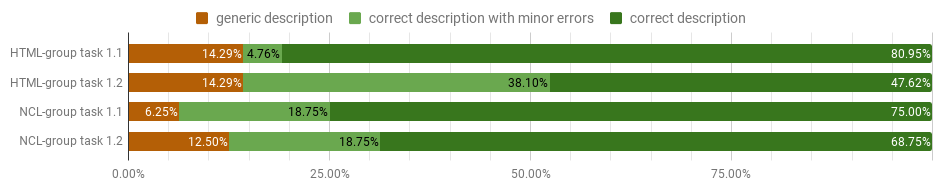
\includegraphics[width=14cm, keepaspectratio]{img/img20.png}
    \captionvspace
	\caption{Participants’ answers in the blocks-based tasks 1.1 and 1.2.}
	\label{fig:blocks-res1}
    \captionvspace
\end{center}
\end{figure}

The answers for the creation tasks were classified as: “correct”, when the
participant correctly made the required block changes; “correct block but with
mirror errors”, when the participant made errors such as forgetting to stop or
start some recognizer, or kept using the selection interaction; and “fail”, when
the changes did not solve what was asked.

\begin{figure}[!ht]
\begin{center}
	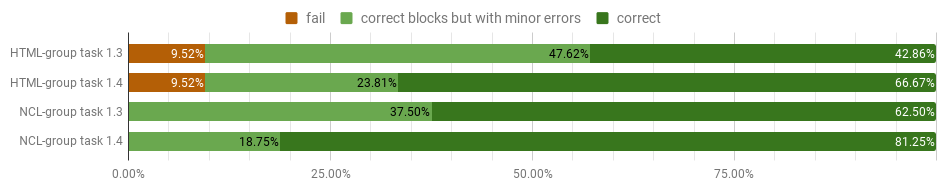
\includegraphics[width=14cm, keepaspectratio]{img/img21.png}
    \captionvspace
	\caption{Participants’ answers in the blocks-based tasks 1.3 and 1.4.}
	\label{fig:blocks-res2}
    \captionvspace
\end{center}
\end{figure}

Page 5 asks the participants’ opinion on TAM statements, as follows.
\fig{fig:blocks-res3} illustrates the participants’ answers.

\begin{itemize}
	\item PU 1: “The concepts presented allow to quickly specify multimodal
	applications.”
	\item PU 2: “The concepts presented allow you to specify multimodal
	applications with quality.”
	\item PU 3: “In general, the concepts presented are useful for specifying
	multimodal applications.”
	\item PEU 1: “The concepts presented are simple and understandable.”
	\item PEU 2: “The concepts presented are easy to learn.”
	\item PEU 3: “In general, the concepts presented are easy to use.”
\end{itemize}

\begin{figure}[!ht]
\begin{center}
	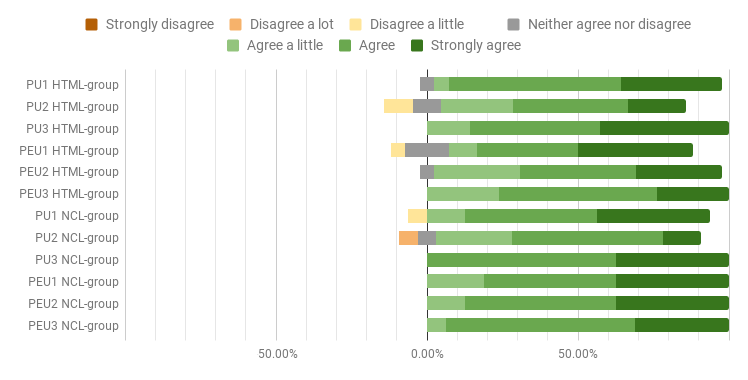
\includegraphics[width=14cm, keepaspectratio]{img/img22.png}
    \captionvspace
	\caption{Participants’ TAM answers about the block-based representation.}
    \captionvspace
	\label{fig:blocks-res3}
\end{center}
\end{figure}

\subsection{Results about extended language}
\label{sec:evaluation:lang-res}

Page 6 presents the syntax representations for the participant’s group language.
It is organized in four sections; each one presents concepts, followed by a
task.

\begin{itemize}
	\item Concepts 2.1: Presents \textit{Media} and \textit{Relationship} elements
	in the extended language syntax and a usage example. The usage example is the
	same as the one in Concepts 1.1.
	\item Task 2.1: Asks the participant to describe a hypervideo application
	presented in the extended language syntax, using \textit{Media} and
	\textit{Relationship} elements. The application is the same as the one in Task
	1.1.
	\item Concepts 2.2: Presents \textit{Recognizer} in the extended language
	syntax and usage example. The usage example is the same as the one in Concepts
	1.2.
	\item Task 2.2: Asks the participant to describe a simple hypervideo
	application, now using a Recognizer in the extended language syntax. The
	application is the same as the one in Task 1.2.
	\item Concepts 2.3: Presents the \textit{CompoundCondition} in the extended
	language syntax and a usage example. The usage example is the same as the one
	in Concepts 1.3.
	\item Tasks 2.3: Asks the participant to develop a new hypervideo application
	in the extended language syntax, now using a \textit{Recognizer} and a
	\textit{CompoundCondition}. The application is the same as the one in Task
	1.3.
	\item Concepts 2.4: Presents \textit{UserClass} in the extended language
	syntax and a usage example. The usage example is the same as the one in
	Concepts 1.4.
	\item Tasks 2.4: Asks the participant to develop a new hypervideo application,
	now using a \textit{UserClass} in the extended language syntax. The
	application is the same as the one in Task 1.4.
\end{itemize}

Regarding the tasks, participants in both groups made few mistakes in both
description (\fig{fig:lang-res1}) and creation tasks (\fig{fig:lang-res2}).

\begin{figure}[!ht]
\begin{center}
	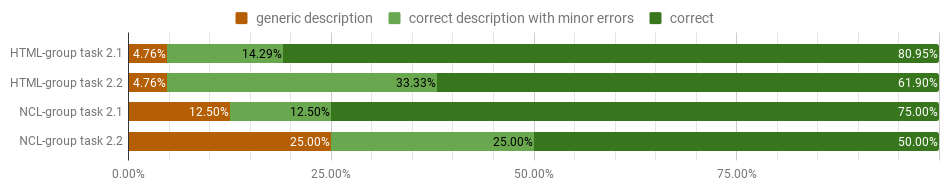
\includegraphics[width=14cm, keepaspectratio]{img/img23.png}
    \captionvspace
	\caption{Participants’ answers in the extended language tasks 2.1 and 2.2}
    \captionvspace
	\label{fig:lang-res1}
\end{center}
\end{figure}

\begin{figure}[!ht]
\begin{center}
	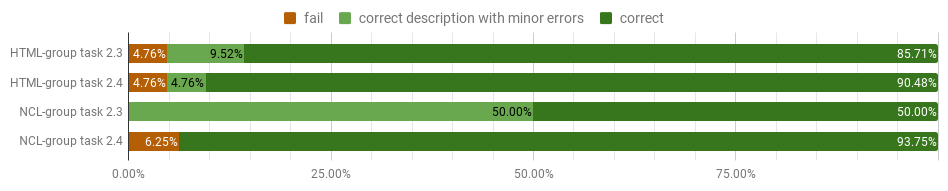
\includegraphics[width=14cm, keepaspectratio]{img/img24.png}
    \captionvspace
	\caption{Participants’ answers in the extended language tasks 2.3 and 2.4.}
    \captionvspace
	\label{fig:lang-res2}
\end{center}
\end{figure}

Page 7 asks the participants’ opinion on TAM statements, as follows.
\fig{fig:lang-res3} illustrates the participants’ answers.

\begin{itemize}
	\item PU 1: “The extended language allows rapid development of multimodal
	applications.”
	\item PU 2: “The extended language allows the development of multimodal
	applications with quality.”
	\item PU 3: “In general, the extended language is useful for the development
	of multimodal applications.”
	\item PEU 1: “The extended language is simple and understandable.”
	\item PEU 2: “The extended language is easy to learn.”
	\item PEU 3: “Overall, the extended language is easy to use.”
\end{itemize}

\begin{figure}[!ht]
\begin{center}
	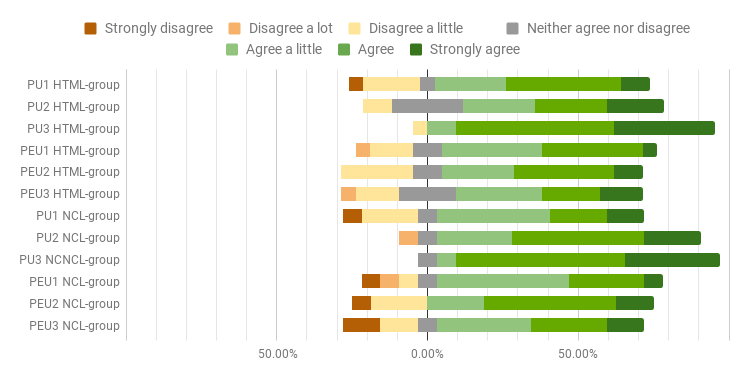
\includegraphics[width=14cm, keepaspectratio]{img/img25.png}
    \captionvspace
	\caption{Participants’ TAM answers about the extended language.}
    \captionvspace
	\label{fig:lang-res3}
\end{center}
\end{figure}

Finally, we asked their opinion regarding the quality of our instantiation with
the statement “The concepts presented in the previous section are clearly
instantiated in the extended language”. \fig{fig:lang-res4} illustrates the
participants’ answers.

\begin{figure}[!ht]
\begin{center}
	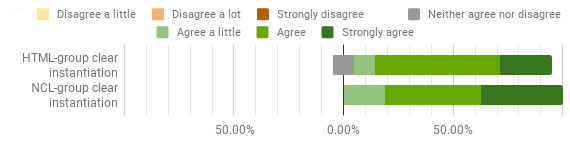
\includegraphics[width=10cm, keepaspectratio]{img/img26.png}
	\caption{Participants’ answers about the concepts instantiation.}
    \captionvspace
	\label{fig:lang-res4}
\end{center}
\end{figure}

\section{Discussion}
\label{sec:evaluation:discussion}

First, we must highlight that we have not found a relation between the users who
had not developed multimodal applications and the ones who performed the tasks
with errors. Also, we have not found relation between users who self-reported to
have lower knowledge of their group language and the ones who performed the
extended language tasks with errors.

If participants had performed the tasks with more errors, it might indicate that
they had not clearly understood the proposed entities and their TAM answer would
not be very informative. However, in general, both NCL and HTML participants
performed the tasks, on both block-based and extended language representations,
with few errors, so their TAM answers can be considered valuable.

Regarding the task identification errors, the most common ones were related with
missing the stop or start of some recognizer. This issue may be related with the
fact that NCL and HTML currently support mouse/key interactions through some
callback function (\textit{e.g.} onclick and onSelection), which do not need to be
activated or deactivated, unlike a recognizer.

Although most users said that the entities were clearly instantiated
(\fig{fig:lang-res4}), their answers to the TAM questions showed a little
difference between the block-based and extended languages representations. The
participants gave some slightly more positive answers for the block-based ones.
To understand why this was the case we need to conduct further studies.